\section{Introduction}
\label{chap:introduction}

%===============================================================
\subsection{Context and Motivation}
%===============================================================

The idea for this thesis came from the ETH spinoff Manukai AG where they need synthetic CAD training data for their machine learning models for CAM manufacturing. Currently they do this using heuristics, generating random sequences of extrusions. Additionally they need to finetune their models on small customer CAD datasets. The companies dont want to share their propietary CAD data beyond their personal applications, as it might contain trade secrets, so Manukai needs to finetune their models with very limited data each time anew to avoid leakage between companies. Here it would be very useful to be able to generate similar high-quality data, which is where this project comes in.

The initial Idea of using a diffusion model following BrepGen \cite{Xu2024brepgen} was postponed as for two main reasons. Firstly, in between the first discussion of the project and the start, another student at Manukai had already explored BrepGen \cite{Xu2024brepgen} and did not come to useful results. Secondly, a new paper was published by the main author of this paper, called AutoBrep \cite{Xu2025autobrep}, which had more promising results. It generated B-Rep's with higher quality and higher complexity Fig \ref{fig:validity} which could be reproduced during inference aswell.

\begin{figure}[h!]
	\centering
	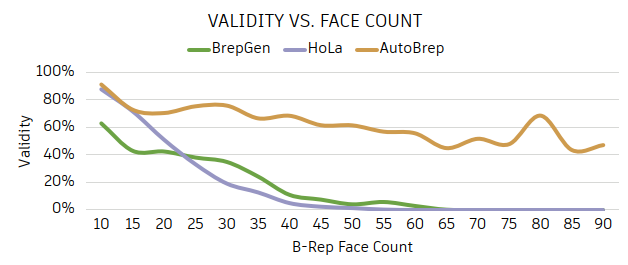
\includegraphics[width=0.6\textwidth]{figures/validity.png}
	\caption{Training and Validation Loss Over Epochs}
	\label{fig:validity}
\end{figure}


%===============================================================
\subsection{Problem Statement}
%===============================================================

Machine learning models for CAD geometry generation have been developed, including the state-of-the-art AutoBrep model, which uses transformer-based architectures to generate Boundary Representations (B-Reps) autoregressively. However, applying such models to new, specialized design domains presents significant challenges:

\par

\textbf{Key challenges:}
\begin{itemize}
    \item \textbf{Domain Adaptation}: Pre-trained models reflect patterns from their training data; specialized design domains (e.g., specific mechanical parts, architectural elements) may have unique characteristics not well-represented in general training corpora
    \item \textbf{Limited Data}: High quality CAD data which is B-Rep compatible is scarce and expensive. It exists in large quantities in industrial companies, but often as parts of trade secrets, and is created in work-intensive manual work by experts.
\end{itemize}

%===============================================================
\subsection{Thesis Objective}
%===============================================================

This work addresses these challenges by investigating \textit{parameter-efficient fine-tuning} of generative CAD models using Low-Rank Adaptation (LoRA). The core research question is:

\par

\textbf{``Can large pre-trained generative CAD models like AutoBrep from \cite{Xu2025autobrep} be efficiently adapted to specialized design domains with limited data using Low Rank Adaptation?''}

To answer this, we:
\begin{enumerate}
    \item Implement a complete pipeline for LoRA-based fine-tuning of the AutoBrep model
    \item Demonstrate domain-specific adaptation on custom CAD datasets
    \item Analyze scalability of multiple LoRA adapters for different domains
    \item Evaluate practical utility and limitations of the approach
\end{enumerate}

%===============================================================
\subsection{Contributions}
%===============================================================

This thesis makes the following contributions to the field of generative design and machine learning for CAD:

\par

\begin{enumerate}
    \item \textbf{Practical Framework}: An end-to-end implementation of LoRA fine-tuning for AutoBrep, including data preprocessing, training, and inference pipelines

    \item \textbf{Efficiency Analysis}: Empirical demonstration whether domain-specific performance can be achieved with only $\approx$1\% additional trainable parameters and order of 500 samples, enabling fine-tuning with very limited data and without changing the base model's parameters

    \item \textbf{Reproducibility}: Detailed documentation of hyperparameters, code, training curves and experimental procedures enabling future research and practical adoption
\end{enumerate}

%===============================================================
\subsection{Thesis Structure}
%===============================================================

The remainder of this thesis is organized as follows:

\begin{itemize}
    \item \textbf{Chapter~\ref{chap:background}}: Background and related work on B-Reps, generative models for CAD, LoRA, and related domain adaptation techniques

    \item \textbf{Chapter~\ref{chap:methodology}}: Detailed methodology covering AutoBrep architecture, LoRA integration, data preprocessing, and training procedures

    \item \textbf{Chapter~\ref{chap:results}}: Experimental results including training convergence, quantitative evaluation, and qualitative analysis of generated models

    \item \textbf{Chapter~\ref{chap:discussion}}: Discussion of findings, limitations, and directions for future research

    \item \textbf{Chapter~\ref{chap:conclusion}}: Summary of contributions and practical implications
\end{itemize}
